We implemented our method
and compared it with the older ones.
The results are very promising.

\section{Connected Component}
\begin{itemize*}
\item {Case 1 All separate graph.}
Input:
1, 2
3, 4
5, 6
7, 8

Output:
8	7
4	3
1	1
5	5
3	3
6	5
2	1
7	7
\end{itemize*}


\begin{figure}[htbf]
\begin{center}
\begin{tabular}{cc}
     % uncomment the next lines, and give the right ps files
     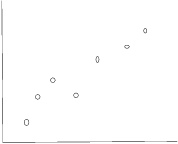
\includegraphics[width=0.3\textwidth]{FIG/data.png} &
     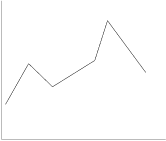
\includegraphics[width=0.3\textwidth]{FIG/plot.png} \\
     %\psfig{figure=FIG/plot.ps,width=2in} \\
     % \psfig{figure=FIG/data.ps,width=2in} &
     % \psfig{figure=FIG/plot.ps,width=2in} \\
    (a) & (b) 
\end{tabular}
\caption{A fictitious dataset (a) and its performance plot (b)}
\label{fig:results}
\end{center}
\end{figure}

